\clearpage
\vspace*{\stretch{2}}
\begin{center} \huge { \textbf{
     Link Prediction on Social Graph}} 
\end{center}
\vspace{\stretch{3}}
\clearpage
\section*{Problem Statement}
The link prediction (LP) problem is to predict future relationships from a given snapshot of a social network. E.g., one may wish to predict that a user will like a movie or book, or that two researchers will coauthor a paper, a user will endorse another on LinkedIn, or two users will become “friends” on Facebook. Apart from the obvious recommendation motive, LP can be useful in social search, such as Facebook Graph Search, as well as ranking goods or services based on not only real friends’ recommendations but also that of imputed social links.

\section*{Popular approaches}
Jaccard : The Jaccard index, also known as the Jaccard similarity coefficient (originally coined coefficient de communauté by Paul Jaccard), is a statistic used for comparing the similarity and diversity of sample sets. The Jaccard coefficient measures similarity between finite sample sets, and is defined as the size of the intersection divided by the size of the union of the sample sets
\begin{equation}
J(A,B) = \frac{\left\vert A \cap B \right\vert}{\left\vert A \cup B \right\vert}
\end{equation}
(If A and B are both empty, we define J(A,B) = 1.) Clearly,
$0 \leq J(A,B) \leq 1$
The MinHash min-wise independent permutations locality sensitive hashing scheme may be used to efficiently compute an accurate estimate of the Jaccard similarity coefficient of pairs of sets, where each set is represented by a constant-sized signature derived from the minimum values of a hash function.\\
The Jaccard distance, which measures dissimilarity between sample sets, is complementary to the Jaccard coefficient and is obtained by subtracting the Jaccard coefficient from 1, or, equivalently, by dividing the difference of the sizes of the union and the intersection of two sets by the size of the union:
Adamic Adar:To decide if nodes u and v may get linked, one strong signal is the number of common neighbors they already share. Adamic and Adar (AA) [1] refined this by a weighted counting: common neighbors who have many other neighbors are dialed down in importance:
\begin{equation}
SIM_{i,j}^{AA} = \sum_{k \in \Gamma(i) \cap \Gamma(j)} \frac{1}{\log {d(k)}}
\end{equation}
where d(k) is the degree of common neighbor k. The AA and RA predictors both penalize the contribution of high-degree common neighbors.


\section*{Our approach}
Unlike AA and other node-pair signals, our new approach recognizes that propensity of linkage is not purely a function of node similarity; it changes with neighborhood. Also, the presence or absence of edge (u, v) rarely determined by nodes far from u and v. So use a edge and triangulated dissimilarity based approach.


\section*{Defining edge dissimilarity}
Let $\Gamma(u)$ be the (immediate) neighbors of u. We will model the edge dissimilarity between u and v as
\begin{equation}
\Delta_{w}(u,v) = w_{uv} . |\Theta_u - \Theta_v|
\end{equation}
 $w_{uv}$ is the weight vector fitted locally for u, v. 
 
\section*{Triangulated Dissimilarity}
The optimization program outputs $w_{uv}^{\ast}$, from which we can compute 
\begin{equation}
\delta_{uv} = w_{uv}^{\ast} . |\Theta_u - \Theta_v|
\end{equation}
Using only this may not be useful for learning a global consistent model. Therefore, we also compute the triangulated dissimilarity
\begin{equation}
\Delta_{w_{xy}}^{x,y} = \sum_{x \in Q,y \in Graph} \frac{\sum_{i \in T(x) \cap T(y)} \Delta_{w_{xy}}(i,x) + \Delta_{w_{xy}}(i,y)}{ |T(x) \cap T(y)|}
\end{equation}
Finally we use this as the score metric,
\begin{equation}
f(u,v)[LL] = \Delta_{w^{*}}(u,v) - \delta_{u,v}
\end{equation}

\section*{Objective function selection}
We assume that the value of the dissimilarity function is low for node pairs which have an edge connecting them and relatively higher for node pairs which are not neighbours. Under these impositions, we wish to minimize the sum of the dissimilarity values of x and y with their common neighbours. This is because this minimization would in turn give the maximum possibility of an edge between x and y that may appear in future. So our objective is to find optimal w, so that the triangulated dissimilarity
\begin{equation}
\Delta^{x,y} = min_{w} \Delta_{w}^{xy}
\end{equation}
is minimized.
\\
Apart from that we want to chose the w vectors in such a manner that $\delta_{uv}$ is larger than nodes which are known to be connected and also smaller than the nodes. So in both cases we can form our constraints in the following manner
\begin{equation}
\sum_{i \in \Gamma(x) \setminus \Gamma(y)} \Delta_{w} (i,x) \leq \alpha \Delta_{w}^{xy}
\end{equation}
\begin{equation}
\sum_{i \in \Gamma(y) \setminus \Gamma(x)} \Delta_{w} (i,y) \leq \alpha \Delta_{w}^{xy}
\end{equation}
\begin{equation}
\sum_{i \in \Gamma(y) \setminus \Gamma(x)} \Delta_{w} (i,x) \geq \alpha \Delta_{w}^{xy}
\end{equation}
\begin{equation}
\sum_{i \in \Gamma(x) \setminus \Gamma(y)} \Delta_{w} (i,y) \geq \alpha \Delta_{w}^{xy}
\end{equation}
So to find the $w$ for the $\delta_{uv}$ computation we can use the constraints as constraints of an SVM. Because as we are trying to minimize the $|w|^2$ which is a classic QP optimization wrt some linear constraints but as our equations can be approximated as SVM constraints (i.e. approximating $ \leq 0$ as $\leq -1$ and $\geq 0$ as $\geq 1$). So for each query-node pair we can run an SVM and find the required $w$ vector.
\\
Similarly minimizing the triangulated dissimilarity is exactly a classic LP problem wrt to the given constraints. We can then simply compute the actual triangulated dissimilarity for the query-node pair and compute the final score.



\section*{Scoring Metric}
We may use only the QP, LP or both approach together. However the meaning of triangulated dissimilarity and edge dissimilarity remains same by same. So the less we get edge dissimilarity the more they link is likely to exist. Also if some nodes triangulated dissimilarity is large then they are well dissimilar with same set of nodes which gives us a signal that they may be similar and we may expect a link indeed. So if the combined score defined as 
$f(u,v)[LL] = \Delta_{w^{*}}(u,v) - \delta_{u,v}$ is large then we are very likely to get links in future.

\section*{Evaluation}
We basically tested on held out data. We sampled the Neighbors and Non Neighbors in .8 or .9 fraction. Then we send the sampled Information to the Recommendation module which analyzes the network based on the given information and comes up with the scores for all query-node pairs. Then for each query we compute the precision and recall and then for all query we compute the MAP.

\section*{MAP, Recall, Precision }
In LP, a separate ranking is produced for each node q from a set of nodes $Q$, which are  therefore called query nodes. Fix a $q$ and consider the ranking of the other $N - 1$ nodes. Some of these are indeed neighbors (or will end up becoming neighbors). Henceforth, we will call $q$’s neighbors as good nodes $G(q)$ and non-neighbors as bad nodes $B(q)$.Ideally, each good node should rank ahead of all bad nodes. precision (also called positive predictive value) is the fraction of retrieved instances that are relevant, while recall (also known as sensitivity) is the fraction of relevant instances that are retrieved. In simple terms, high precision means that an algorithm returned substantially more relevant results than irrelevant, while high recall means that an algorithm returned most of the relevant results.

First we define at query node q the quantity
\begin{equation}
Avp(q) = \frac{1}{L} \sum_{k = 1}^{N-1} P_{q}(k) r_{q}(k)
\end{equation}
as Average Precision where $N - 1$ is the number of nodes excluding the query node itself, $L$ is the number of retrieved relevant items and $r_{i} (k)$ is an indicator taking value 1 if the item at rank $k$ is a relevant item (actual neighbor) or zero otherwise (non-neighbor). Averaging further over query nodes. Using this we compute the overall Mean Average Precision.

\section*{Integrated Single Stage Learning}
In both LP and QP based approach though we are using the help of the neighborhood, but in every query-node computation, when we are going to compute both edge and reference dissimilarity we are using their own weight vector i.e. for different query-node pair even in computing the same dissimilarity. One way to encounter this is to use an integrated one step learning approach. Instead of learning for a specific query-node pair we try to learn all query-node pair together. But the main drawback in this approach is problem with scaling. If the graph is in the order of thousands of nodes then depending the query size and feature vector size the QP and LP problems can be in the size (number of variables) of millions. So solving them is not a very practical idea indeed. So we are trying to keep both the essence. Instead of learning the whole graph together we can use a per query based learning or may also define a threshold on number of variables. Whenever the quota is filled we solve the LP and QP problems and then go on solving the rest. Though this decouples the theoretical QP and LP problems still we can do some experimentation.

\section*{Implementing the Integrated Approach}
To use the integrated approach we need to map the variables due to different each query-node pair in a single variable space. We can formally define the process with an example. Suppose we have,
\\Undirected Graph: in adjacency Matrix form $G = (V, E), |V| = n$
\\Feature Data $(F)$: for each node of the graph we have a feature vector of some give dimension.
\\Query Data $(Q)$: A set of vertexes in $V$for which will run learn together.
Now suppose we have the part of the network in Figure~\ref{fig:Sample Network},
\begin{figure}
\centering
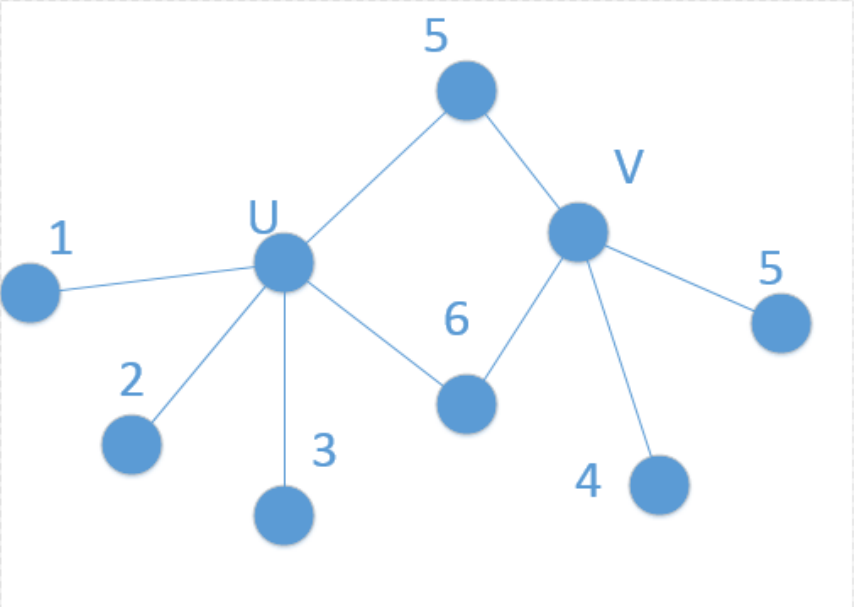
\includegraphics[width=\textwidth,height=\textheight,keepaspectratio]{link_prediction/images/network.png}
\caption{Sample Network}
\label{fig:Sample Network}
\end{figure}

Now according to our problem formulation, the linear constraints after SVM like approximations  are,
\begin{equation}
W_{uv}^T \frac{T_{u1} + T_{u2} + T_{u3}}{3} - W_{uv}^T \frac {T_{u5} + T_{u6}+T_{v5} + T_{v6}}{4} \leq -1 
\end{equation}
\begin{equation}
W_{uv}^T \frac{T_{v4} + T_{v5}}{2} - W_{uv}^T \frac {T_{u5} + T_{u6}+T_{v5} + T_{v6}}{4} \leq -1 
\end{equation}
\begin{equation}
W_{uv}^T \frac{T_{u4} + T_{u5}}{2} - W_{uv}^T \frac {T_{u5} + T_{u6}+T_{v5} + T_{v6}}{4} \geq 1 
\end{equation}
\begin{equation}
W_{uv}^T \frac{T_{v1} + T_{v2} + T_{v3}}{3} - W_{uv}^T \frac {T_{u5} + T_{u6}+T_{v5} + T_{v6}}{4} \geq 1 
\end{equation}

So from these equations (total $|Q| * |V| * 4$ constraints) for each query-node pair  we want to find the $W_{uv}$ for all query $u$ and node $v$ together. So we try the bring all the equations in the same variable space and we want to find a W vector of dimension $|F|*|Q|*|V|$, [Where $|F|$ is the feature dimension]\\
i.e. our $$W = [W_{q1,1} W_{q1,2} ... W_{q1,|V|} W_{q2,1} W_{q2, 2} ... W_{q2,|V|}... W_{q_{|Q|},1} W_{q_{|Q|}, 2} ... W_{q_{|Q|}, |V|}]$$
So we can define the mapping as
\begin{equation}
W_{uv} [k] \rightarrow (i*|V|+v)*|F| + k 
\end{equation}
, where $u$ is the $ith$ query node.
So now if we use the QP based approach then our objective function will be
\begin{equation}
\sum_{x \in Q, y \in V} |W|_{xy}^2
\end{equation}
and for the LP based approach it will be
\begin{equation}
\sum_{x \in Q,y \in Graph} \Delta_{w_{xy}}^{x,y} = \sum_{x \in Q,y \in Graph} \frac{\sum_{i \in T(x) \cap T(y)} \Delta_{w_{xy}}(i,x) + \Delta_{w_{xy}}(i,y)}{ |T(x) \cap T(y)|}
\end{equation}
Now we extract the corresponding weight vector values for each query-node pair and we compute the score with triangulated and edge dissimilarities.

\section*{Why use Pegasos and why it did not work ?}
As our constraints and objective in finding the edge dissimilarity are similar to SVM equations we tried to use PEGASOS which is a very large scale SVM solver. PEGASOS is a stochastic subgradient descent algorithm for solving the optimization problem cast by Support Vector Machines. When we use a linear kernel the algorithm works on a per training example basis and if the required accuracy is $e$ and regularization is $\lambda$, then we get a running time of $O(\frac {d}{\lambda e})$ per example where d is a bound on number of non zero features. So as we have a very large number of equations this algorithm looks particularly suitable for our purpose. But however PEGASOS gives a speedup at the cost of accuracy and we are already approximating our constraints this may not always give a good result. Also in our last approach we used the edge dissimilarity value as the scoring methodology which we may not give good results as described early. so we propose a hybrid variant in next section.

\section*{LP Based approach}
We used the original constraints on a LP solver (GLPK - GNU Linear Programming toolKit - Simplex algorithm). we ran our implementation on the movielens (3952 nodes) data set and our MAP was .53 (which is still not better than the two step learning approach). Here we also used the same weight values for triangulated and edge dissimilarity value computation.

\section*{Results}
We ran our system on the Movie lens data set ( 3952 nodes, 276 queries). Initially we used the one step QP approach. However we got very low MAP. Then we implemented the LP based approach with a limit of number of variables for the problems. Then we got a MAP value of 0.53 which is below the old approach (.70). However we also inverted the scoring which resulted in a poor MAP, which implies that our results are not random. We also plotted(Figure~\ref{fig:precisiondegree} and ~\ref{fig:averageprecisiondegree}) the distribution of the precision values wrt degrees which are promising and shows that it can be improved.
\begin{figure}
\centering
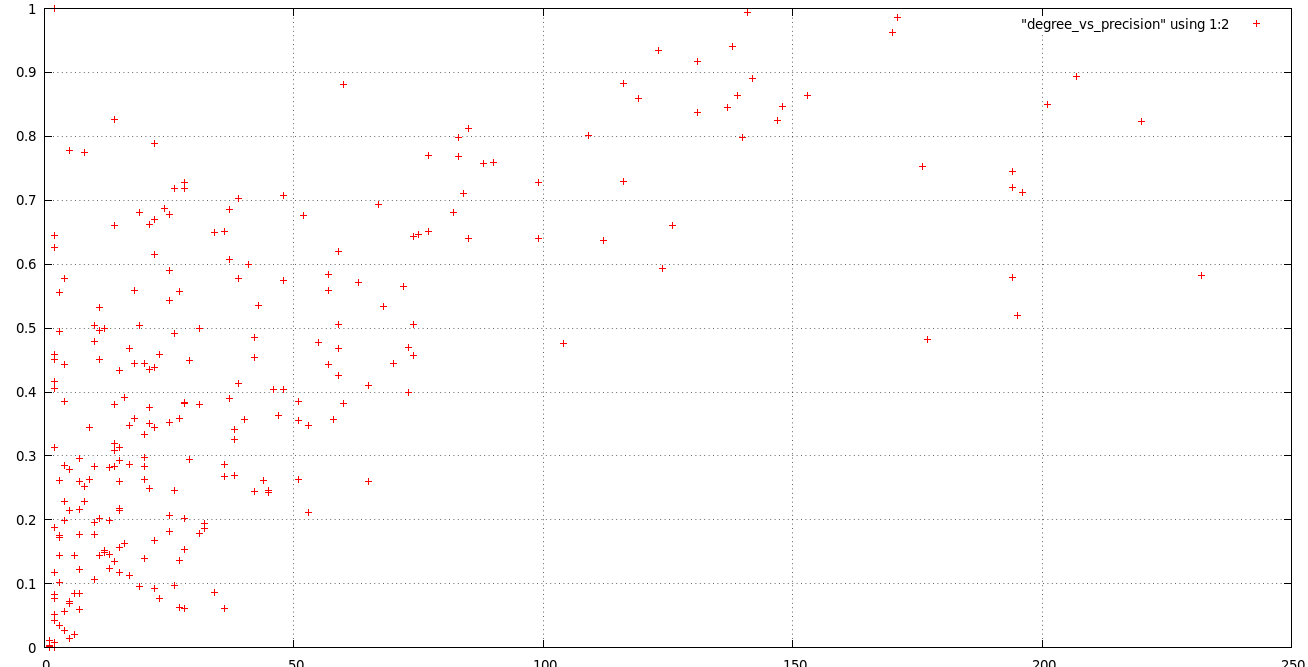
\includegraphics[width=\textwidth,height=\textheight,keepaspectratio]{link_prediction/images/total.png}
\caption{Precision vs Degree}
\label{fig:precisiondegree}
\end{figure}
\begin{figure}
\centering
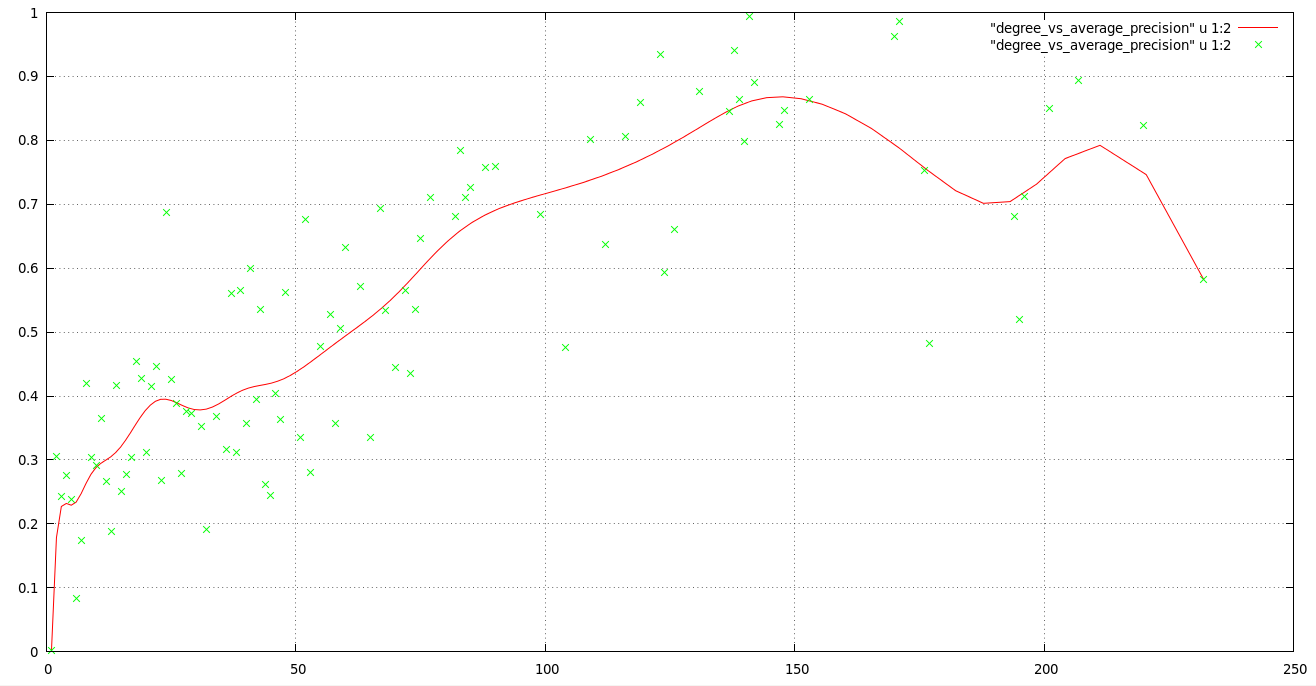
\includegraphics[width=\textwidth,height=\textheight,keepaspectratio]{link_prediction/images/average.png}
\caption{Average Precision vs Degree}
\label{fig:averageprecisiondegree}
\end{figure}

\section*{Proposed Hybrid approach for further experimentation}
The only QP based approach gave very poor result, but however the LP approach gave comparatively better results. So we can use the LP weights in triangulated weight calculations and QP weights in edge dissimilarity calculations which needs further experimentations.
   
%    handler.computeHittingTime = @computeHittingTime;
%    handler.computeCommuteTime = @computeCommuteTime ;
%    handler.computeKatzScore = @computeKatzScore ;
%    handler.computeJaccardScore = @computeJaccardScore ;
%    handler.computeAdamicAdarScore = @computeAdamicAdarScore ;
%    handler.computeCommonNeighborScore = @computeCommonNeighborScore ;
%    handler.computeRootedPageRank = @computeRootedPageRank ;
%    handler.computePreferentialAttachment = @computePreferentialAttachment ;
%    handler.computeSimRank = @computeSimRank ;
%    handler.computeGraphDistance = @computeGraphDistance;
%    handler.computeCommuteTimeFresh = @computeCommuteTimeFresh;
\section*{Adding more features}
After the previous work instead of going to the hybrid approaches as suggested earlier we tried to introduce new featur - Hitting time, Commute Time, Katz Score, Preferential Attachment, Jaccard Score, Adamic Adar, Common Neighbor score and GraphDistance \cite{linkpredsocial}. Here we give a brief overview of the features. After that we have done a quadratic coupling study of features.
% hitting time and commute time
\\
A random walk on $G$ starts at a node $x$ and iteratively moves to a neighbor of $x$ chosen uniformly at random from the set $\Gamma(x)$ (set of direct neighbors of the node $x$). The hitting time $H_{x,y}$ from $x$ to $y$ is the expected number of steps required for a random walk starting at $x$ to reach $y$.Because the hitting time is not in general symmetric, it is also natural to consider the commute time $C_{x,y} := H_{x,y} + H_{y,x}$. From \cite{hittingtime} we find that we can easily compute hitting time matrix $H$ according to the following formula $H = 1 \dot{}  [diag( \widetilde{Z})]^{T} - \widetilde{Z}$ where $\widetilde{Z}$ is the scaled fundamental matrix as defined in \cite{hittingtime}.
\\
%Katz Score
In this work we have also incorporated two new features - Preferential Attachment and Katz Score. Katz Score is among the methods to refine the notion of shortest paths by considering the set of all paths between two nodes. Katz defines a measure that directly sums over this collection of paths, exponentially damped by length to count short paths more heavily. This notion leads to the measure $Score(x,y) := \sum\limits_{l=1}^{\infty} \beta^l |paths_{x,y}^{<l>}|$ where $paths_{x,y}$ is the set of all length- paths from $x$ to $y$, and $\beta > 0$ is a parameter of the predictor (A very small $\beta$ yields predictions much like common neighbors, because paths of length three or more contribute very little to the summation). We can easily find a closed expression of the $Score$ matrix. By definion the $score = \sum\limits_{l=1}^{\infty} \beta^l M^l$ (where M is the adjacency matrix of the graph). Now $Score + I = \sum\limits_{l=0}^{\infty} \beta^l M^l = (I-\beta M)^{-1} \iff Score = (I-\beta M)^{-1} - I$ From the definition of Katz score, as we are considering all possible paths it also captures the notion of the global structure of the Graph.
\\
%Preferentail Attachment Score
Our framework also tries to capture the the local effects by introducing the Preferential Attachment feature. For a node $x$, let $\Gamma (x)$ denote the set of neighbors of $x$. Now the definition of Preferential Attachment comes from the growth model. We know if we introduce a new node then $x$ will be one of its neighbors with probability $|\Gamma(x)|$. Now in our graphs are not temporal and as both $x$ and $y$ already exists so to capture their local similarity be good approach would be to define $PA(x,y) := |\Gamma(x)|.|\Gamma(y)|$.
\\
% common neighbor and graph distance
The common neighbor score is defined as $score(x, y) := |\Gamma(x) \cap \Gamma(y)|$, the number of neighbors that $x$ and $y$ have in common. And graph distance is basically the all pair shortest path distance which we computed using Floyd Warshall Algorithm. For all these methods we have written MATLAB scripts.

\section*{Feature coupling study}
With our earlier work we have introduced a lot of features. But some features may be good for classification and some may be not. Also if we train using forming vectors using only one dimension features then there is high chance that we might miss the correlation effect between features which can be a major signal for the outer level classifier. Also as taking all these experiments would have taken a lot of manual effort so we have completely automated the process of linear and quadratic feature coupling study. Our system takes input of a bit vector for linear features and a bit Matrix for correlation study of features.

\section*{Experimental results}

In Figure~\ref{fig:arbitration_study} we show the linear feature selection study. Here on average we find that if we take the combination of LL (local learning), CC (co-clustering), KM (Katz Measure), PA (Preferential Attachment) and AA (Adamic Adar) then we get best MAP values in all data sets. In Figure~\ref{fig:quad_study} we show the effect of taking the quadratic terms. And we deduce that quadratic combination of the selected features found in linear study gives best performance. Finally in Figure~\ref{fig:precion_recall} study we study the our methodology against leading algorithm and find that our old framework combined with the LL,CC,KM,PA and AA scores gives superior results.
\begin{figure}
\centering
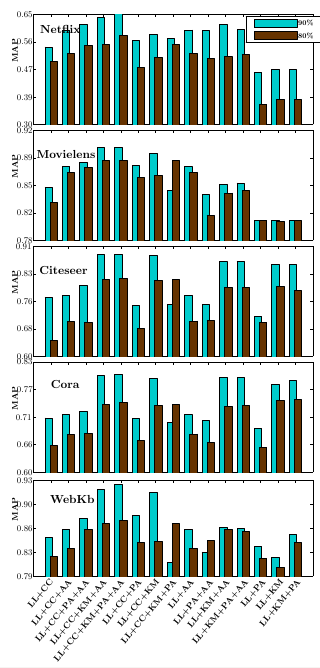
\includegraphics[width=\textwidth,height=\textheight,keepaspectratio]{link_prediction/images/arbitration_study.png}
\caption{Feature Ablation Study with 90\% and 80\% Sampling}
\label{fig:arbitration_study}
\end{figure}

\begin{figure}
\centering
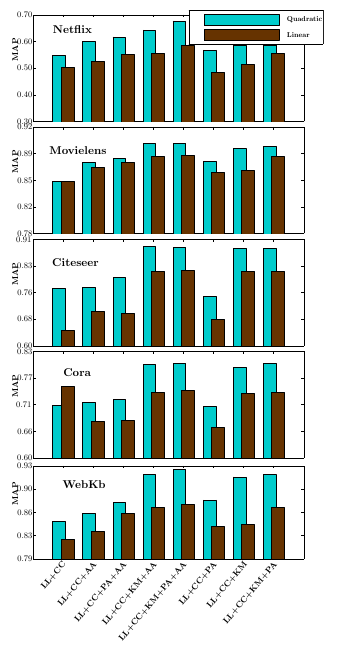
\includegraphics[width=\textwidth,height=\textheight,keepaspectratio]{link_prediction/images/quad_study.png}
\caption{Effect of Quadratic Terms}
\label{fig:quad_study}
\end{figure}

\begin{figure}
\centering
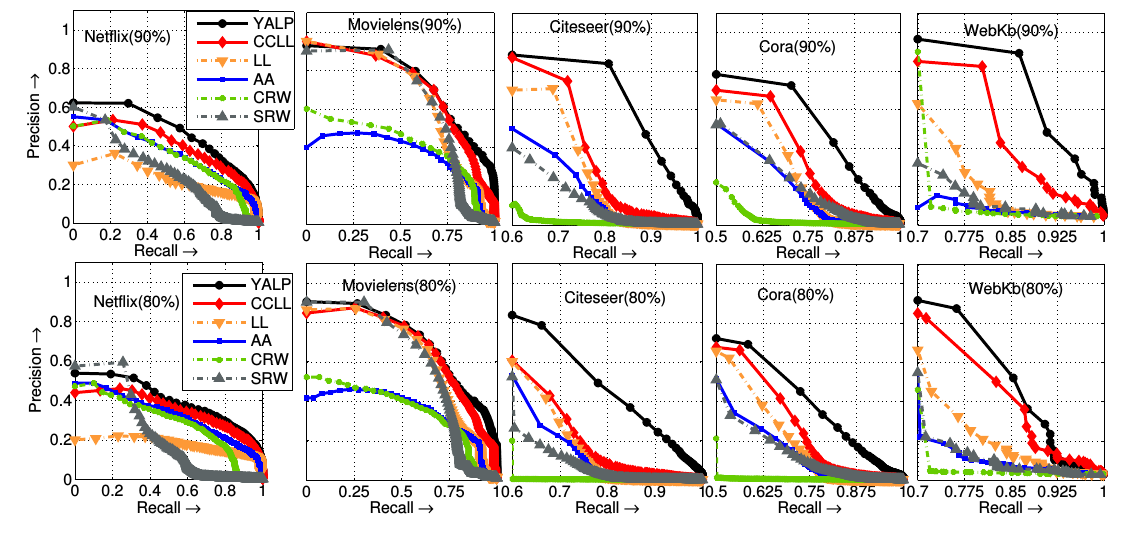
\includegraphics[width=\textwidth,height=\textheight,keepaspectratio]{link_prediction/images/precision_recall.png}
\caption{Precision vs. recall curves for all data sets and algorithms}
\label{fig:precion_recall}
\end{figure}


\section*{Tools Used}
The initial system for LP and QP based score calculation was built using C++ and Boost Graph Library. The later new featurs and feature combination and arbitration study was done entirely in MATLAB. For LP we used the GLPK library and for QP we used PEGASOS.
